\documentclass{article}
\usepackage[utf8]{inputenc}
\usepackage{lipsum} % Used for tableofcontents
\usepackage[parfill]{parskip} % No indent for a new line
\usepackage[capitalise]{cleveref} % cref
\usepackage{mwe} % used for minipages to show two figures side by side
\usepackage{subcaption}
\usepackage{enumitem}
\usepackage{cite}
\usepackage{graphicx}
\usepackage{float}
\usepackage[margin=1.5in]{geometry}
\graphicspath{{./figures/}}


\title{ACML Homework \\ Music by RNNs}
\author{Ibrahim Hadzic (i6200920), Alexander Reisach (i6197692) \\ \textbf{github.com/Scriddie/midi-rnn}}
\date{\today}

\begin{document}
\maketitle

\section{Getting Things Running}
We adapted the code from \textit{https://github.com/brannondorsey/midi-rnn} to tensorflow 2.1, and ran some experiments with the default settings. As can be seen in \ref{fig:tensorboard_2}, although training loss is steadily decreasing, there is no clear trend visible for the validation performance.

\begin{figure}[H]
    \centering
    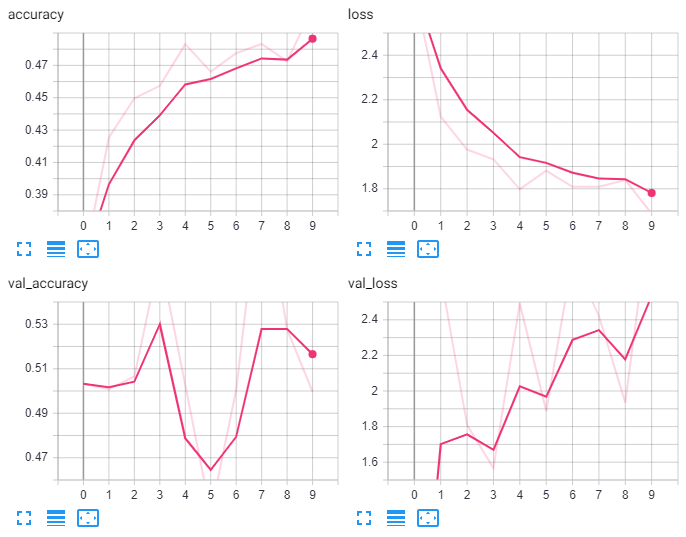
\includegraphics[scale=0.40]{tensorboard_2.png}
    \caption{Tensorboard output for default settings}
    \label{fig:tensorboard_2}
\end{figure}

In order to test different and more computationally intensive settings, we use the Aachen cluster's GPU. We use keras' CuDNNLSTM layers (see file \textit{train\_gpu.py}) instead of regular LSTM layers to take advantage of the accelerated linear algebra (XLA) optimizations.


\section{Experiments}
Ever since the term "random guessing" has come out of fashion, we have specialized in "principled experimentation" instead, and this project is no exception. Following best practices from the internet (c.f. \ref{fig:good_advice}), we experimented in particular with the following parameters:
\begin{itemize}
    \item number of (LSTM) layers and nodes per (LSTM) layer
    \item input window size
    \item numper of training epochs
    \item dropout ratio
\end{itemize}

\begin{figure}[H]
    \centering
    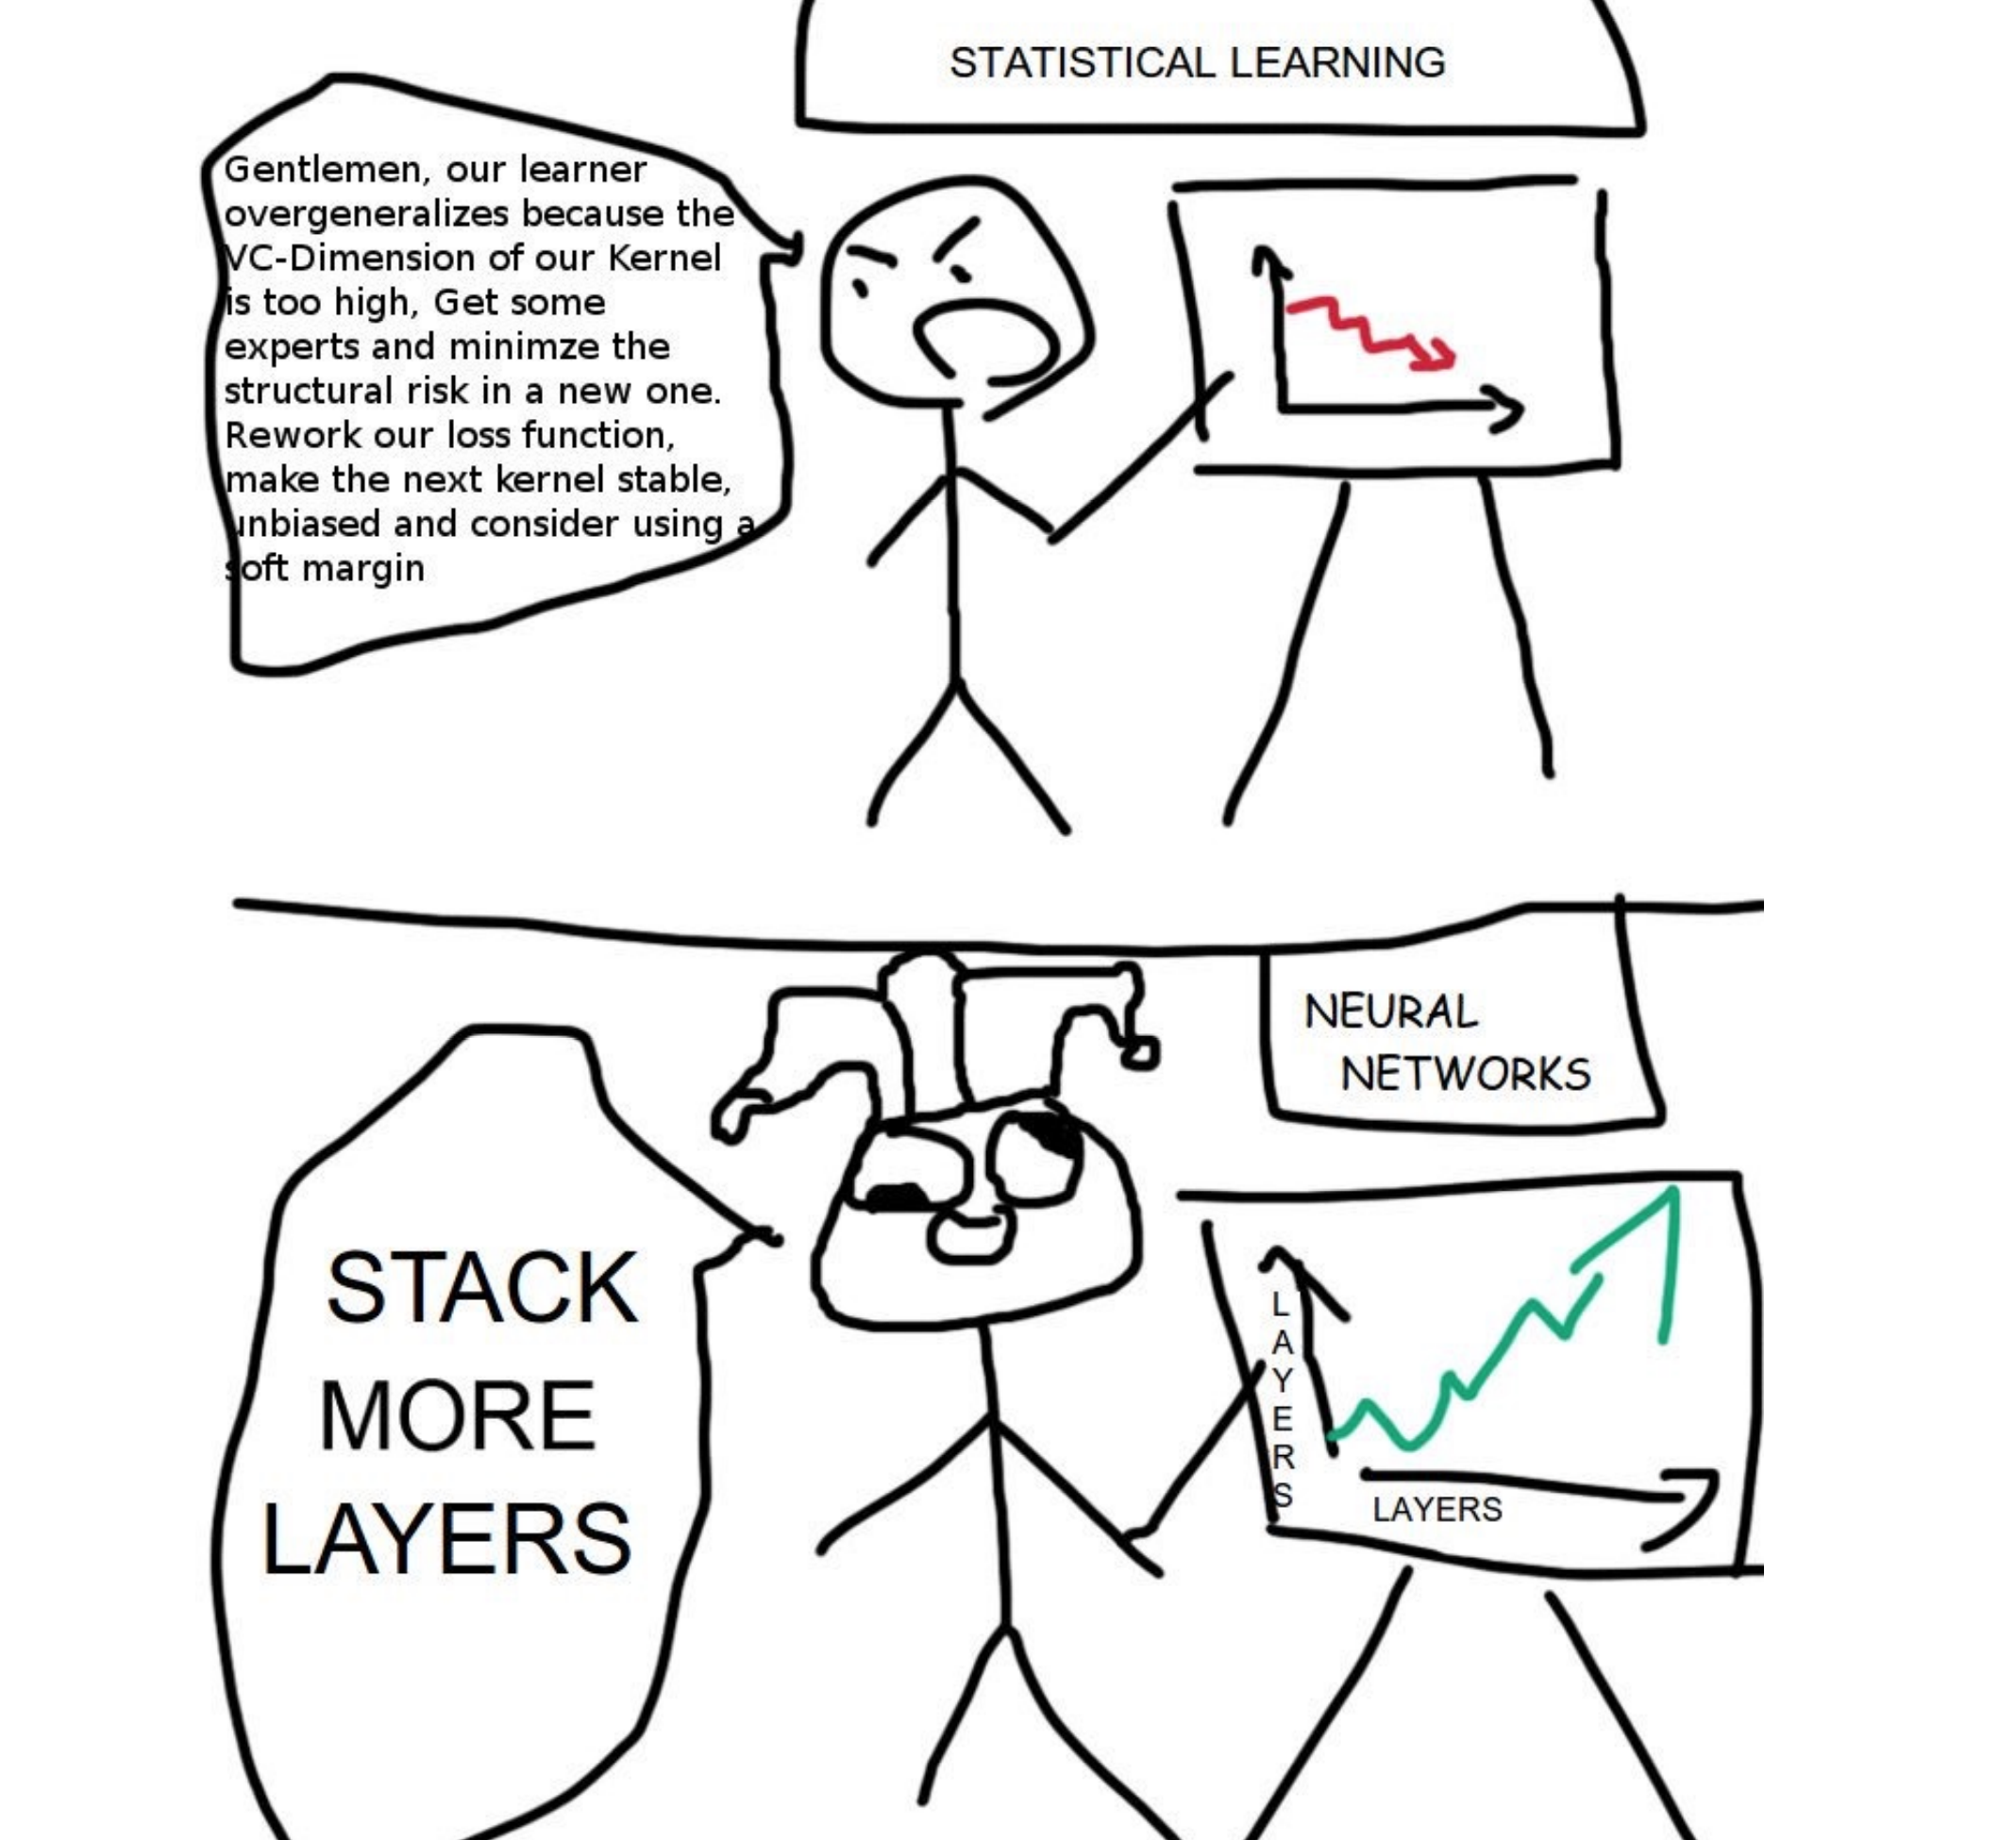
\includegraphics[scale=0.28]{stack_more_layers.png}
    \caption{Good advice from the internet}
    \label{fig:good_advice}
\end{figure}

In this spirit, we ran our model with the following settings:
\begin{figure}[H]
    \centering
    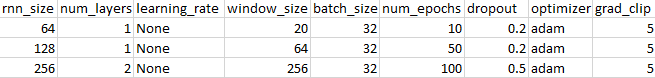
\includegraphics[scale=0.8]{experiment_schedule_2.png}
    \caption{Experiment Schedule}
    \label{fig:experiment_schedule1}
\end{figure}

\section{Results}
All trained models can be found in the folder \textit{cluster\_experiments}. Each model contains a subfolder \textit{generated} with \textit{.mid} files containing model generated output. The first model, trained only for 10 epochs does produce sounds, but they can hardly be called music, and there seem to be frequent "blank spots", where there is no generation at all for a short period of time. The second model, trained for 50 epochs and with a larger hidden layer produces outcomes that sound more melodic and are largely free from "blank spots". The third model (two hidden layers with 256 nodes each for 100 epochs) produces the greatest variety of low-pitched and high-pitched notes. While there are some melodic elements here and there, there is still a huge gap to the original input files. To make sure the model does not only remember songs it has seen during training, we also generated music from a holdout set. We did not notice a difference in musical quality using this input as compared to before.


\end{document}
